% Template: Fabian Wenzelmann, 2019, modified by us
\documentclass{beamer}

\usepackage[utf8]{inputenc}
\usepackage[ngerman]{babel} % use ngerman here for german text
\usepackage[T1]{fontenc}
\usepackage{mathtools}
\usepackage{amssymb}
\usepackage{lmodern}
\usepackage[protrusion=true,expansion=true,kerning]{microtype}
\usepackage{graphicx}
\usepackage{hyperref}
\usepackage{mdframed}
\usepackage{amsrefs}
\usepackage{bm}
\usepackage[center]{caption}

\usepackage{float}

\usetheme{Pittsburgh}
%\usetheme{CambridgeUS}
\usecolortheme{dolphin}

Bildunterschrift
\addto\captionsngerman{%
	\renewcommand{\figurename}{Abb.}%
	\renewcommand{\tablename}{Tab.}%
}

% einige Abkuerzungen
\newcommand{\qenc}{q_{\boldsymbol\phi}(\mathbf{z}|\mathbf{x}_i)}
\newcommand{\qencd}{q_{\phi}(z|x_i}
\newcommand{\penc}{p_{\boldsymbol\theta}(\mathbf{z}|\mathbf{x}_i)}
\newcommand{\pdec}{p_{\boldsymbol\theta}(\mathbf{x}_i|\mathbf{z})}
\newcommand{\C}{\mathbb{C}} % komplexe
\newcommand{\K}{\mathbb{K}} % komplexe
\newcommand{\R}{\mathbb{R}} % reelle
\newcommand{\Q}{\mathbb{Q}} % rationale
\newcommand{\Z}{\mathbb{Z}} % ganze
\newcommand{\N}{\mathbb{N}} % natuerliche
\newcommand{\E}{\mathbb{E}} % Erwartungswert
\newcommand{\F}{\mathcal{F}} 
\newcommand{\G}{\mathcal{G}} 


\newcommand{\tx}{\widetilde{x}}
\newcommand{\tz}{\widetilde{z}}
\newcommand{\tZ}{\widetilde{Z}}
\newcommand{\tX}{\widetilde{X}}
\newcommand{\tmu}{\widetilde{\mu}}
\newcommand{\tsig}{\widetilde{\sigma}}
\newcommand{\bP}{\mathbb{P}}
\newcommand{\bbf}{\bold{f}}
\newcommand{\bmu}{\bm{\mu}}
\newcommand{\bsig}{\bm{\sigma}}
\newcommand{\z}{\mathbf{z}}
\newcommand{\x}{\mathbf{x}_i}

\makeatletter
\newcommand{\vast}{\bBigg@{3}}
\newcommand{\Vast}{\bBigg@{5}}
\makeatother


\title{Missing Data Imputation mit \\Variational Autoencodern}
%\subtitle{sub-überschrift}

% For short you could for example use the last name only, it's optional as is
% the short title
\author{Niklas Brunn, Ben Deitmar, Sebastian Hahn\\Jannis Klingler, Clemens Schächter}

\date{08.02.2021}

% removes the navigation symbols
% often they don't work and I find them rather annoying
\beamertemplatenavigationsymbolsempty{}

% You can have a logo to appear on all slides
 \logo{
\includegraphics[height=1cm]{Bilder/logo}}

\begin{document}
	
	\begin{frame}
		\titlepage
	\end{frame}
	
	

\author[Jannis Klingler]{Nix}


\beamertemplatenavigationsymbolsempty{}

\logo{
\includegraphics[height=1cm]{Bilder/logo}}



\section{Variational Autoencoder}

\begin{frame}
	\frametitle{Beispiel \emph{time series}}
	\begin{figure}[!htbp]
		
\includegraphics[scale=0.25]{Bilder/rotatingMNIST}\\
		Beispiel einer \emph{time series} bestehend aus \\10 Bildern des Datensatzes rotatingMNIST
	\end{figure}
\end{frame}

\begin{frame}
	\frametitle{Modellannahmen}
	Gegeben:
	\begin{itemize}
		\item Datensatz $\textbf{X} = \lbrace\x \rbrace_{i=1}^{N} \subset \R^{D\times N}$
		\item Datenpunkte $\x\sim p(\x)$ (u.i.v. Realisierungen einer hochdimensionalen Zufallsvariable)
	\end{itemize}
\end{frame}

\begin{frame}
	\frametitle{Latente Variablen Modell}
	Suchen:
	\begin{itemize}
		\item Verteilung der Datenpunkte $\x$
		\item Eine niedrigdimensionale Darstellung der Daten, die den Prozess, der die Daten erzeugt, möglichst gut modelliert
		\item Führen dazu \emph{Latente Variablen} $\z$, die auf dem \emph{latenten Raum} $\mathcal{Z} = \R^d$ mit $d\ll D$ definiert sind, ein
	\end{itemize}
\end{frame}

\begin{frame}
	\frametitle{Latente Variablen Modell}
	Das \emph{Latente Variablen Modell} besteht nun aus den Verteilungen:
	\begin{itemize}
		\item Verteilung der Daten $p(\x)$
		\item Posteriorverteilung $p(\z|\x)$
		\item Priorverteilung $p(\z)$
		\item Generatives Modell $p(\x|\z)$
	\end{itemize}
\end{frame}

\begin{frame}
	\frametitle{Latente Variablen Modell}
	Sind interessiert an der Verteilung
	\[p(\x)= \int_{\z} p(\x,\z) \mathrm{d}\textbf{z} = \int_{\z} p(\x|\z)p(\z) \mathrm{d}\z.\]
	\textbf{Problem:} Dieses Integral kann aufgrund der hohen Dimension des Raumes $\mathcal{X}$ und der Komplexität des Modells 
	nicht berechnet und auch nicht sinnvoll approximiert werden. \\ \ 
	\\
	Mit dem Satz von Bayes gilt dies auch für die Verteilung
	\[p(\z|\x)= \frac{p(\x|\z)p(\z)}{p(\x)}.\]
\end{frame}

\begin{frame}
	\frametitle{Implementierung}
		\begin{itemize}
		\item Führen nun das Inferenzmodell $q_{\boldsymbol\phi}(\z|\x)$ ein und suchen die Parameter $\boldsymbol\phi^{*}$ für die $q_{\boldsymbol\phi^{*}}(\z|\x) \approx p_{\boldsymbol\theta}(\z|\x)$ gilt 
		\item In einem Variational Autoencoder werden die Verteilungen $q_{\boldsymbol\phi}(\z|\x)$ und $p_{\boldsymbol\theta}(\x|\z)$ durch neuronale Netze dargestellt und approximiert
		\item Können dann die Verteilung von $p(\z)$ festlegen (häufig $\mathcal{N}(0,\textbf{I})$)
	\end{itemize}
\end{frame}

\begin{frame}
	\frametitle{Schematische Darstellung der VAE-Architektur}
	\begin{figure}[htbp!]
		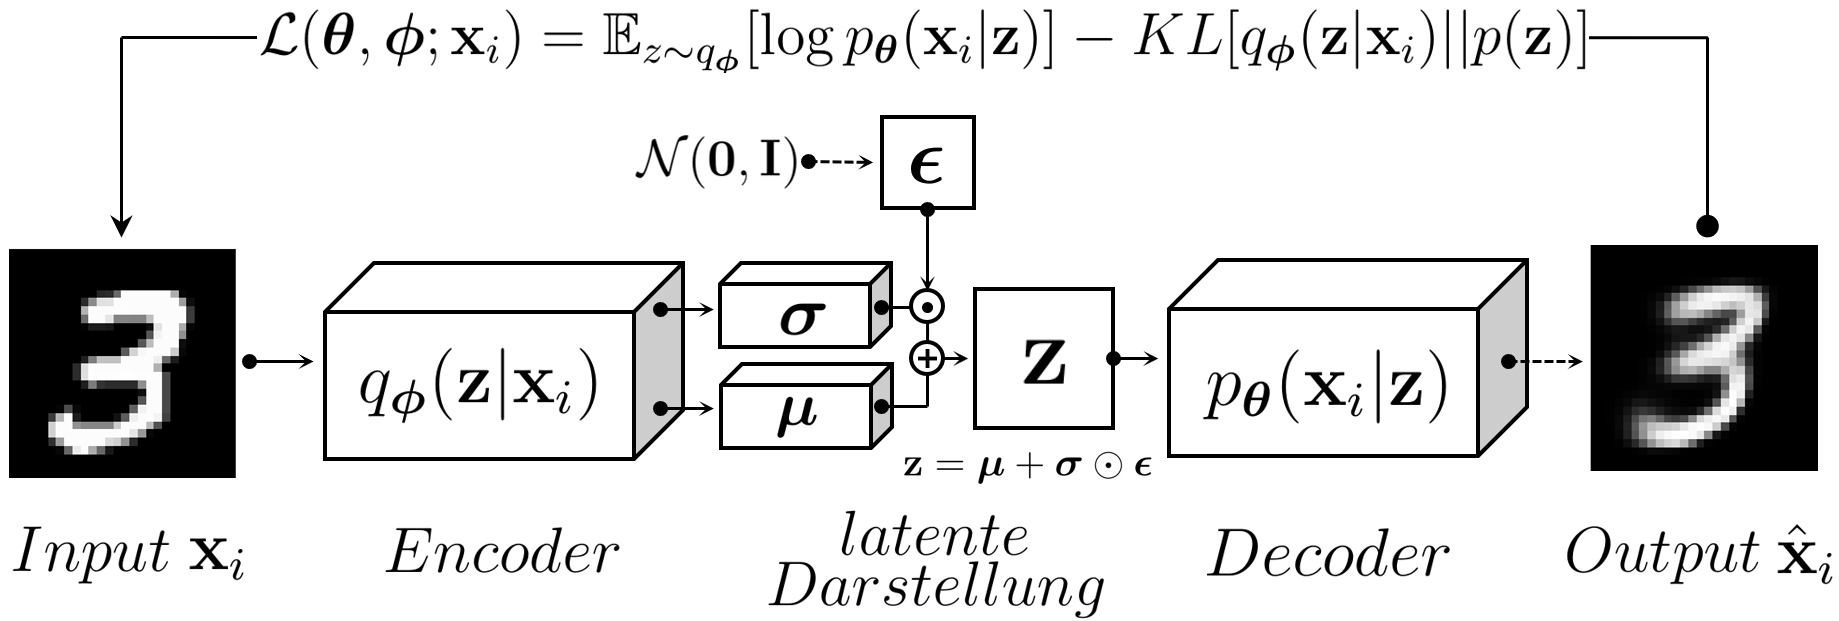
\includegraphics[scale=0.27]{Bilder/VAE-Modell.PNG}
	\end{figure}
\end{frame}
	

\author[Sebastian Hahn]{Nix}


\beamertemplatenavigationsymbolsempty{}

\logo{
\includegraphics[height=1cm]{Bilder/logo}}



\section{Sektion-Überschrift}

\begin{frame}
	\frametitle{Frame-Überschrift}
	Inhalt
\end{frame}

	

\author[Niklas Brunn]{Nix}


\beamertemplatenavigationsymbolsempty{}

\logo{
\includegraphics[height=1cm]{Bilder/logo}}



\section{ODE$^{2}$VAE}

\begin{frame}
    \frametitle{ODE$^{2}$VAE}
    Wir wollen als nächstes \emph{time series} mit einen \emph{ODE$^{2}$VAE} modellieren\\ 
    \text{ }\\
    \text{ }
    \begin{itemize}
    	\item[ ] \emph{ODE$^{\ 2}$VAE: Deep generative second order ODEs with Bayesian neural networks} von Ç. Yıldız, M. Heinonen und H. Lähdesmäki
    \end{itemize}	
\end{frame}




\begin{frame}
	\frametitle{Idee}
	\begin{itemize}
	\item Bewegungen (z.B. Fadenpendel) lassen sich nicht gut mit einem Standard-VAE modellieren\\
	\item \textbf{neuer Ansatz:} Zeitliche Abhängigkeit der Daten berücksichtigen und die Bewegung durch Differentialgleichungen zweiter Ordnung (ODE$^{2}$) modellieren 
	\item \textbf{Vorteile:} Wir können so zu beliebigen Zeitpunkten abfragen und auch Prognosen für die Zukunft generieren
	\end{itemize}
\end{frame}



\begin{frame}
    \frametitle{Notation}
    \begin{itemize}
    	\item Eine \emph{time series} $\mathbf{x}_{0:T}=(\mathbf x_{0}, \mathbf x_{1}, \ldots,\mathbf x_{T})\in \mathbb{R}^{D\times T}$ zu beobachteten Zeitpunkten $t_{0}, t_{1},\ldots,t_{T}$\\
    	\item \textbf{Annahme:} Zeitliche Änderung der latenten Darstellung kann stetig durch eine ODE$^{2}$ beschrieben werden\\
    	\item Zugehörigen latenten Zustände zu den beobachteten Zeitpunkten sind $\mathbf z_{0:T}=(\mathbf z_{0}, \mathbf z_{1}, \ldots, \mathbf z_{T})\in \mathbb{R}^{d\times T}$\\ 
    	\item Latente Zustände werden in Positions- und Geschwindigkeitskomponente aufgeteilt $\mathbf z_{t}=(\mathbf s_{t}, \mathbf v_{t})$
    \end{itemize}
\end{frame}




\begin{frame}
\frametitle{Notation}
    \begin{itemize}
    	\item Die ODE$^{2}$ lässt sich als ein System zweier ODE$^{1}$ schreiben
    \end{itemize}	
    {\footnotesize\begin{align*}
	    \dfrac{\partial^2 \mathbf{z}(t)}{\partial^2 t}=f_{\boldsymbol{\psi}}\left(\mathbf{z}(t), \tfrac{\partial \mathbf{z}(t)}{\partial t}, t\right)%, \\
	    %&\begin{cases*}
	    %\tfrac{\partial \mathbf{s}(t)}{\partial t}=\mathbf v(t) \\
	    %\tfrac{\partial \mathbf{v}(t)}{\partial t}=f_{\boldsymbol{\psi}}(\mathbf s(t), \mathbf v(t), t) \\
	    %\end{cases*}
	\end{align*}}
    \begin{itemize}
    	\item $f_{\boldsymbol{\psi}}$ ist dabei ein NN, welches das Beschleunigunsfeld erlernt
    	\item Lösen des Anfangswertproblems in $\mathbf{z}_{0}=(\mathbf{s}_{0}, \mathbf{v}_{0})$ liefert zu beliebigen Zeitpunkten $T$ eine Lösung
	\end{itemize}
    {\footnotesize\begin{align*}
    \left(\begin{array}{cc}
    \mathbf s_{T} \\
    \mathbf v_{T}
    \end{array}\right)
    =
    \left(\begin{array}{cc}
    \mathbf s_{0} \\
    \mathbf v_{0}
    \end{array}\right)
    +
    \int_{0}^{T}
    \left(\begin{array}{cc}
    \mathbf v(t) \\
    f_{\boldsymbol{\psi}}(\mathbf s(t), \mathbf v(t), t)
    \end{array}\right)
    \mathrm{d}t.
    \end{align*}}
\end{frame}




\begin{frame}
\frametitle{Modell}
Das Modell besteht aus den folgenden Komponenten:
\begin{itemize}
	\item Als \textbf{Prior} für die latente Ausgangsposition $p(\mathbf{s}_{0})$ und die latente Ausgangsgeschwindigkeit $p(\mathbf{v}_{0})$ wird eine Standardnormalverteilung gewählt
	\item Einem \textbf{Position-Encoder} welcher mit $\mathbf{x}_{0}$ die erste latente Ausgangsposition $\mathbf{s}_{0}$ encodiert und einem \textbf{Velocity-Encoder} welcher mit den ersten $m\geq2$ Werten $\mathbf{x}_{m}$ die latente Ausgangsgeschwindigkeit encodiert\\
    \item Einem \textbf{ODE-Netzwerk} welches zu einem Anfangswert eine Kurve im latenten Raum bestimmt\\
    \item Einem \textbf{Decoder}, welcher die aus der Kurve resultierenden latenten Positionen decodiert
\end{itemize}
\end{frame}




\begin{frame}
    \frametitle{Modell}
    	\begin{figure}[h!]
    	\centering
    	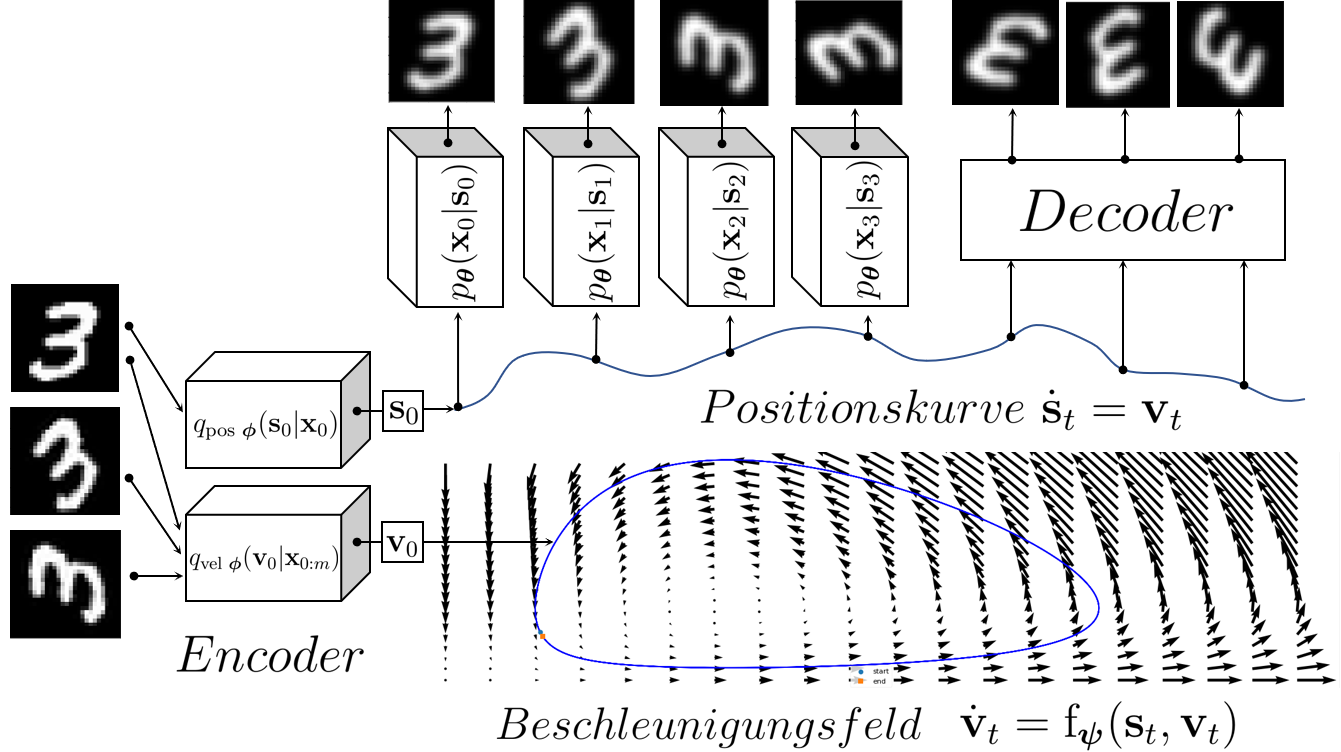
\includegraphics[scale=0.36]{Bilder/ODE2VAE_ODE_Net}
    \end{figure}
\end{frame}




\begin{frame}
    \frametitle{Training}
    Als Trainingskriterium verwenden wir erneut die \textbf{ELBO} 	
    	{\footnotesize\begin{align*}
            \log\big(p_{\boldsymbol{\theta}}(\mathbf{x}_{0:T})\big)&\ge \E_{\mathbf{z}_{0:T}\sim q_{\boldsymbol\phi,\boldsymbol\psi}}
            \left[\log\big(p_{\boldsymbol\theta}\left(\mathbf{x}_{0:T}|\mathbf{z}_{0:T}\right)\big)\right] - D_{KL}\big[q_{\boldsymbol\phi,\boldsymbol\psi}(\mathbf{z}_{0:T}|\mathbf{x}_{0:m})||p_{\boldsymbol\theta,\boldsymbol\psi}(\mathbf{z}_{0:T})\big]\\
            &=\underbrace{\E_{\mathbf{z}_{0}\sim q_{\text{enc }\boldsymbol\phi}}
    	    \left[\log\big(p_{\boldsymbol\theta}\left(\mathbf{x}_{0}|\mathbf{z}_{0}\right)\big)\right] - D_{KL}\big[q_{\text{enc }\boldsymbol\phi}(\mathbf{z}_{0}|\mathbf{x}_{0:m})||p_{\boldsymbol\theta}(\mathbf{z}_{0})\big]}_{\text{Vanilla-VAE ELBO}}\\ &+ \underbrace{\sum_{t=1}^T \E_{\mathbf{z}_{t}\sim q_{\text{ode }\boldsymbol\psi}}
    	    \left[\log\big(p_{\boldsymbol\theta}\left(\mathbf{x}_{t}|\mathbf{z}_{t}\right)\big)\right] - D_{KL}\big[q_{\text{ode }\boldsymbol\psi}(\mathbf{z}_{t}|\mathbf{x}_{0:m})||p_{\boldsymbol\theta,\boldsymbol\psi}(\mathbf{z}_{t})\big]}_{\text{dynamic loss}}
    \end{align*}}
    Während dem Training sieht das Modell alle Inputframes einer \emph{time series}
\end{frame}


\begin{frame}
    \frametitle{Ergebnisse}
    \emph{bouncing Balls}
    \begin{figure}[!htbp]
    	\centering
    	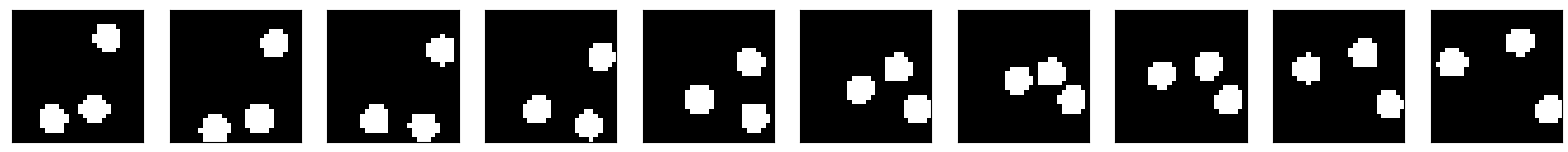
\includegraphics[scale=0.28]{Bilder/bouncingBalls}
    \end{figure}
\end{frame}




\begin{frame}
\frametitle{Ergebnisse}
\textbf{Von links nach rechts:} Modellinput, tatsächlicher Versauf der \emph{time series}, Rekonstruktionen 
\begin{figure}[h!]
	\begin{minipage}{0.135\textwidth}
		%\begin{mdframed}[style=innersmall]
			\center{}
			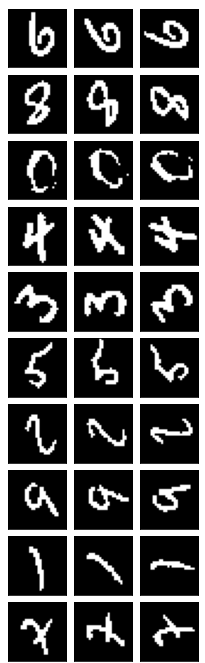
\includegraphics[scale=0.19]{Bilder/MNISTorig1}
			%\center{}
			%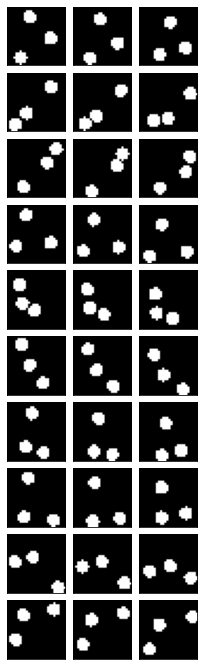
\includegraphics[scale=0.15]{Bilder/bouncingBalls_ODEorig1}
		%\end{mdframed}
	\end{minipage}
	\begin{minipage}{0.33\textwidth}
		%\begin{mdframed}[style=innersmall]
			\center{}
			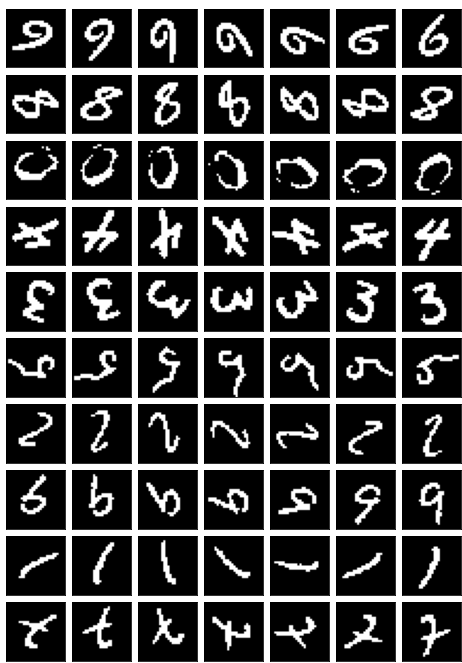
\includegraphics[scale=0.19]{Bilder/MNISTorig2}
			%\center{}
			%
\includegraphics[scale=0.15]{Bilder/bouncingBalls_ODEorig2}
		%\end{mdframed}
	\end{minipage}
	\begin{minipage}{0.33\textwidth}
		%\begin{mdframed}[style=innersmall]
			\center{}
			
\includegraphics[scale=0.19]{Bilder/MNISTrec}
			%\center{}
			%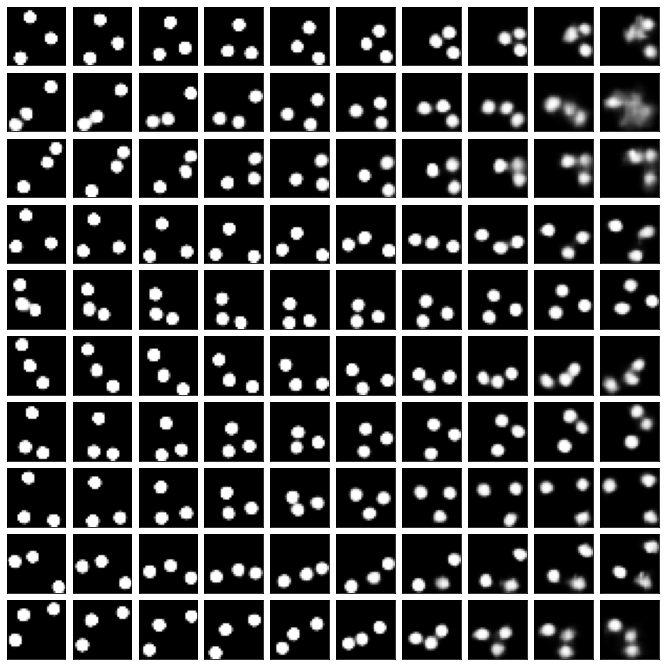
\includegraphics[scale=0.15]{Bilder/bouncingBalls_ODE}
		%\end{mdframed}
	\end{minipage}
\end{figure}
\end{frame}




\begin{frame}
\frametitle{Ergebnisse}
\textbf{Von links nach rechts:} Modellinput, tatsächlicher Versauf der \emph{time series}, Rekonstruktionen 
\begin{figure}[h!]
	\begin{minipage}{0.135\textwidth}
		%\begin{mdframed}[style=innersmall]
		%\center{\small{Modellinput}\vspace{0.1cm}}
		%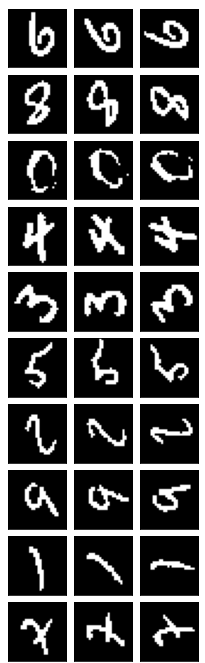
\includegraphics[scale=0.15]{Bilder/MNISTorig1}
		\center{}
		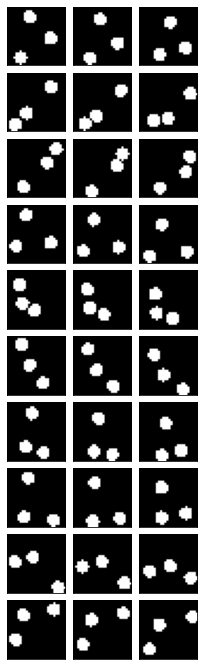
\includegraphics[scale=0.19]{Bilder/bouncingBalls_ODEorig1}
		%\end{mdframed}
	\end{minipage}
	\begin{minipage}{0.33\textwidth}
		%\begin{mdframed}[style=innersmall]
		%\center{Groundtruth\vspace{0.1cm}}
		%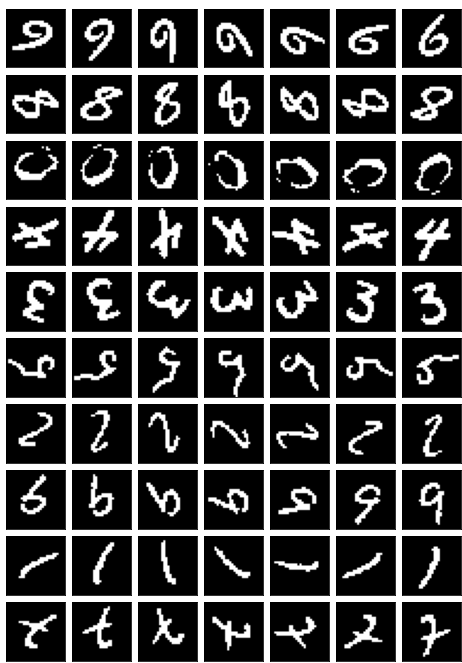
\includegraphics[scale=0.15]{Bilder/MNISTorig2}
		\center{}
		
\includegraphics[scale=0.19]{Bilder/bouncingBalls_ODEorig2}
		%\end{mdframed}
	\end{minipage}
	\begin{minipage}{0.33\textwidth}
		%\begin{mdframed}[style=innersmall]
		%\center{Rekonstruktion}
		%
\includegraphics[scale=0.15]{Bilder/MNISTrec}
		\center{}
		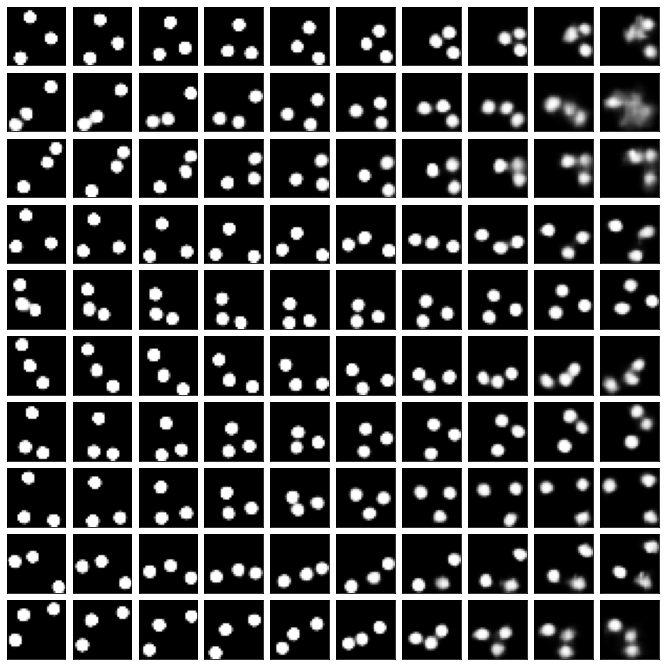
\includegraphics[scale=0.19]{Bilder/bouncingBalls_ODE}
		%\end{mdframed}
	\end{minipage}
\end{figure}
\end{frame}




\begin{frame}
\frametitle{Ergebnisse}
\emph{AVI-Motion}
\begin{figure}[!htbp]
	\centering
	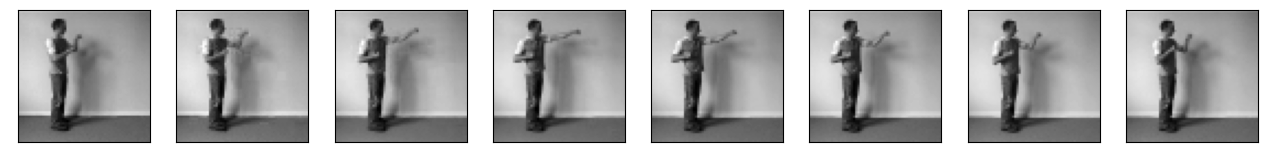
\includegraphics[scale=0.35]{Bilder/AVIMotion}
\end{figure}
\end{frame}




\begin{frame}
\frametitle{Ergebnisse}
\begin{figure}[h!]
	\begin{minipage}[position=l]{0.5\textwidth}
		%\begin{mdframed}[style=inner]
			\center{Modellinput\vspace{0.1cm}}
			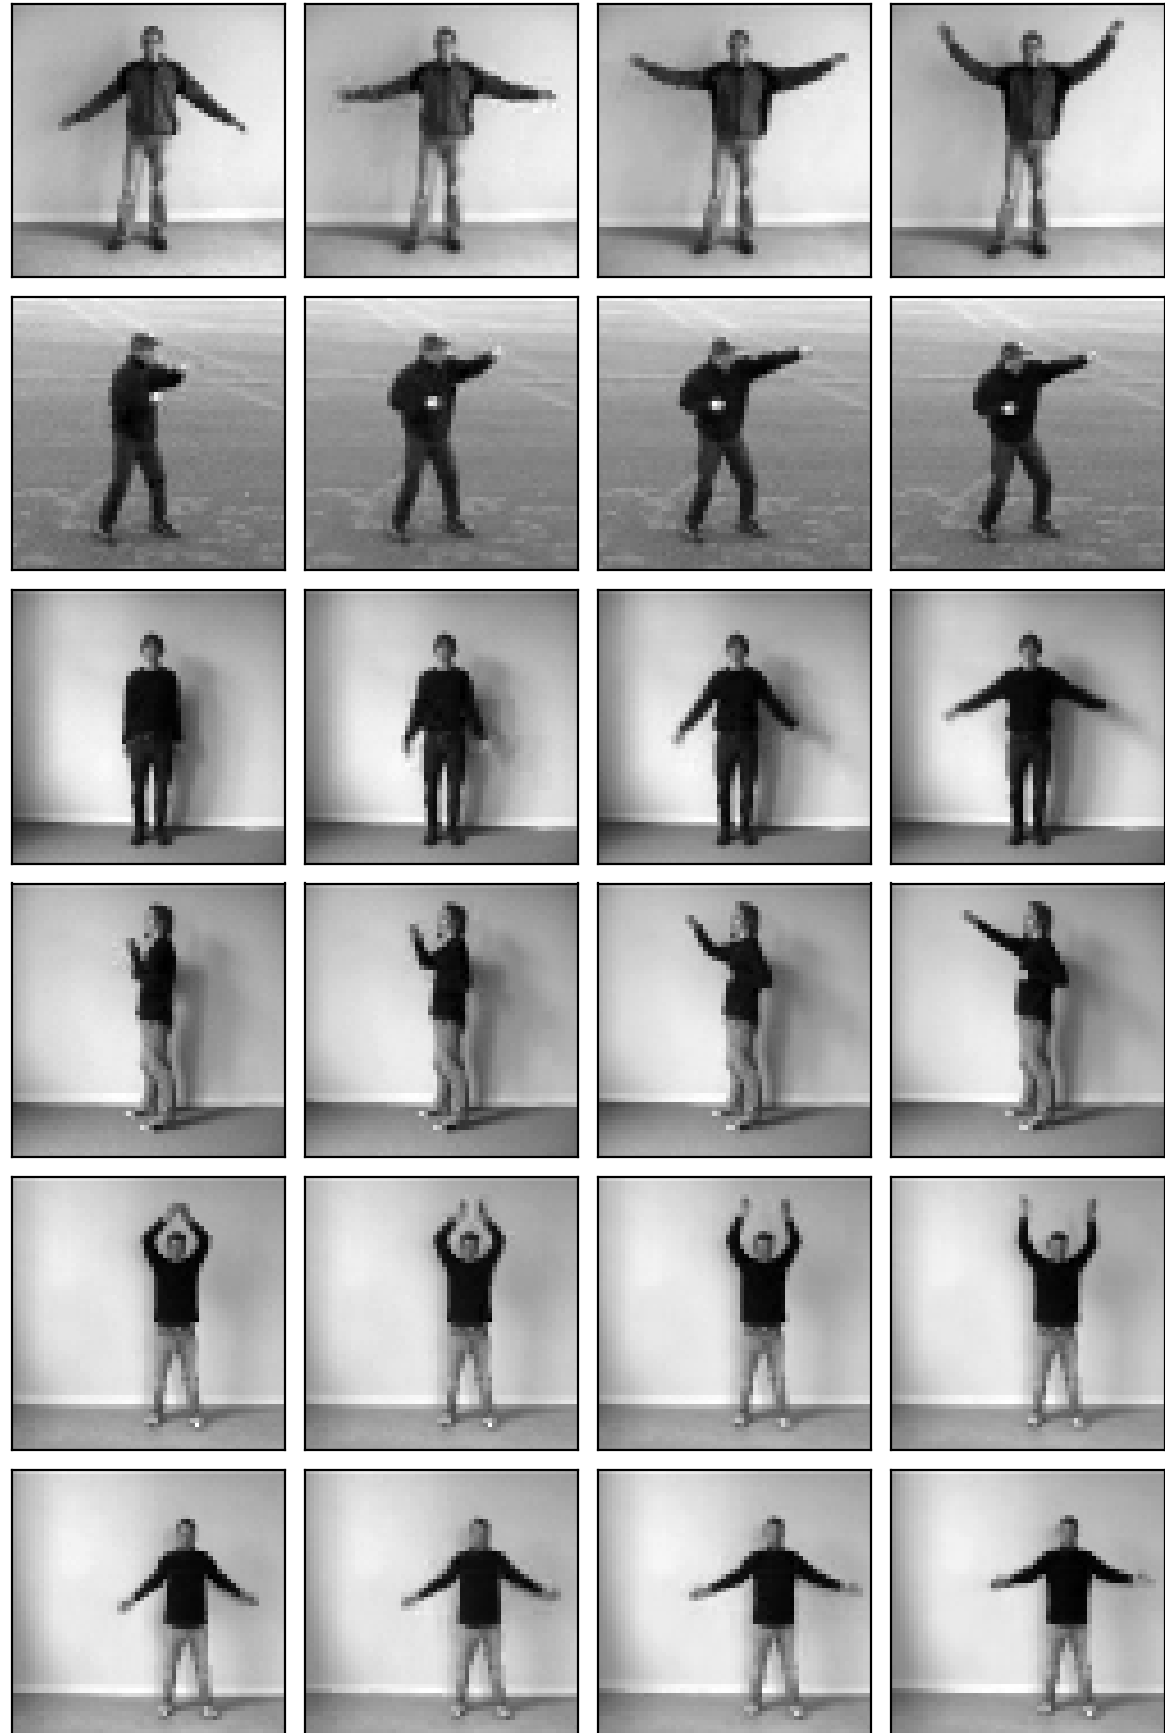
\includegraphics[scale=0.3]{Bilder/movies_input}
		%\end{mdframed}
	\end{minipage}
	\begin{minipage}[position=r]{0.4\textwidth}
		%\begin{mdframed}[style=inner]
			\center{Extrapolation\vspace{0.1cm}}
			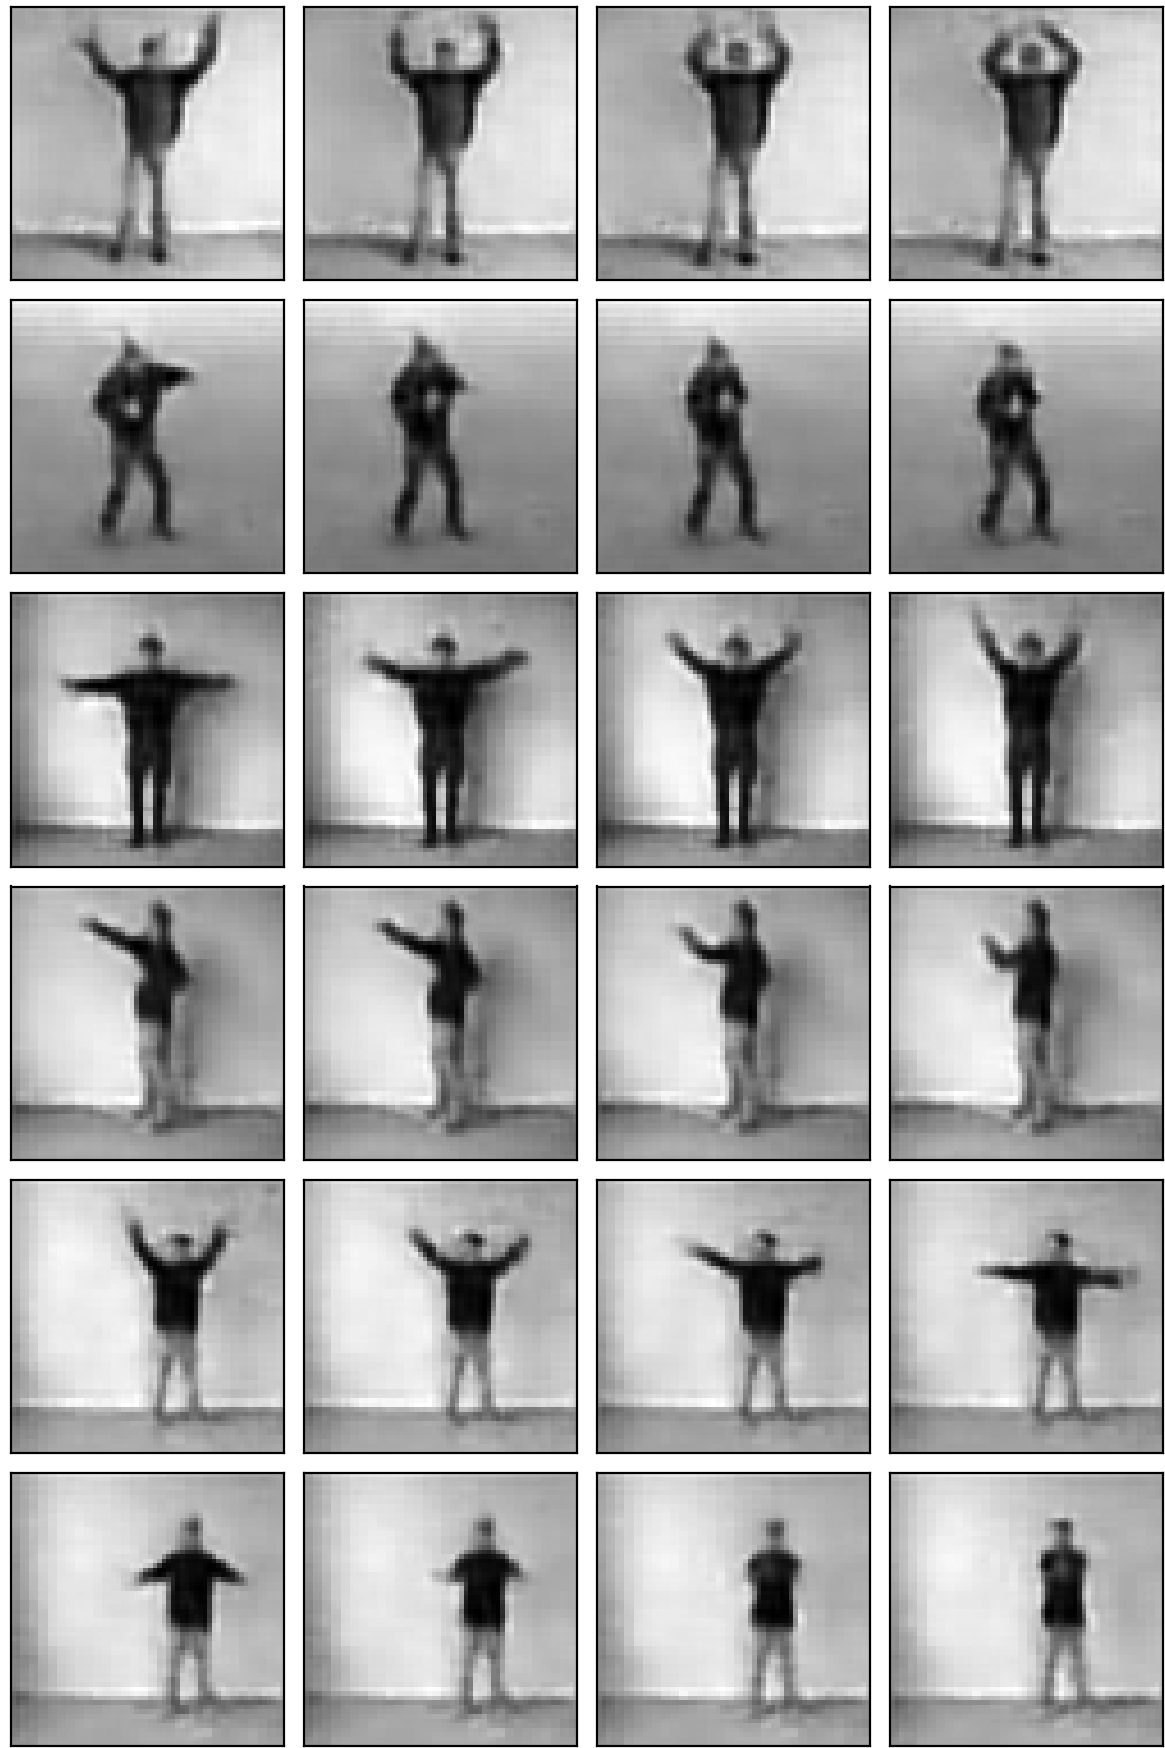
\includegraphics[scale=0.298]{Bilder/movies_extrapolation}
		%\end{mdframed}
	\end{minipage}
\end{figure}
\end{frame}


	
	

\author[Ben Deitmar]{Nix}


\logo{
\includegraphics[height=1cm]{Bilder/logo}}


\section{SDE$^M$VAE}

\begin{frame}
	\frametitle{Erste Verallgemeinerung: ODE M-ter Ordnung}
	Bisherige ODE:
	\begin{align*}
	\nabla s(\cdot,\omega) &= v(\cdot,\omega) \in \R^d\\
	\nabla v(\cdot,\omega) &= \bold{f}\big(s(\cdot,\omega),v(\cdot,\omega)\big) \in \R^d
	\end{align*}
	Verallgemeinerung für $M=3$:
	\begin{align*}
	\nabla s(\cdot,\omega) &= \bold{f}_1\big(s(\cdot,\omega),v(\cdot,\omega),w(\cdot,\omega)\big)\\
	\nabla v(\cdot,\omega) &= \bold{f}_2\big(s(\cdot,\omega),v(\cdot,\omega),w(\cdot,\omega)\big)\\
	\nabla w(\cdot,\omega) &= \bold{f}_3\big(s(\cdot,\omega),v(\cdot,\omega),w(\cdot,\omega)\big)
	\end{align*}
	Schreibe $\bm{\mu} = \bold{f} : \R^{M \times d} \rightarrow \R^{M \times d}$ und $z = (s,v,w)^T \in \R^{M \times d}$.
\end{frame}


\begin{frame}
	\frametitle{Zweite Verallgemeinerung: SDE}
	Bisherige ODE: \ \ $\forall k < M, \forall i \leq d :$
	\begin{align*}
	 & d z^{(k,i)}(t) = \bm{\mu}^{k,i}(z(t)) \, dt
	\end{align*}
	Verallgemeinerung für $\bm{\sigma} : \R^{M \times d} \rightarrow \R^{M \times d \times n}$:
	\begin{align*}
	& d z^{(k,i)}(t) = \bm{\mu}^{k,i}(z(t)) \, dt + \sum\limits_{j=1}^n \bm{\sigma}^{k,i,j}\big(z^{(0)}(t),...,z^{(M-1)}(t)\big) \, dW^j_t
	\end{align*}
	\rotatebox[origin=c]{180}{$\Lsh$} $(M \, d)$-dimensionale SDE mit Brownschen Bewegungen (BBs) $W^1,...,W^n$.
\end{frame}


\begin{frame}
	\frametitle{BB als Random Walk}
	\begin{itemize}
		\item Satz von Donsker:\\
		Seien $Y_1,Y_2,...$ uiv. mit $\E[Y_i]=0$ und $\sigma^2 := \E[Y_i^2] < \infty$.\\
		Definiere den Prozess
		\begin{align*}
		& W_{m,t} := \frac{1}{\sqrt{m}} \left( \sum\limits_{i=1}^{\lfloor mt \rfloor} Y_i + (mt - \lfloor mt \rfloor) Y_{\lfloor mt \rfloor +1}\right) \in C^0([0,\tau]) \ .
		\end{align*}
		Dann gilt $W_{m,\cdot} \xrightarrow{m \rightarrow \infty}_{\mathcal{L}} W$ (BB) in $C^0([0,\tau])$.
		
		\item Anschaulich:\\
		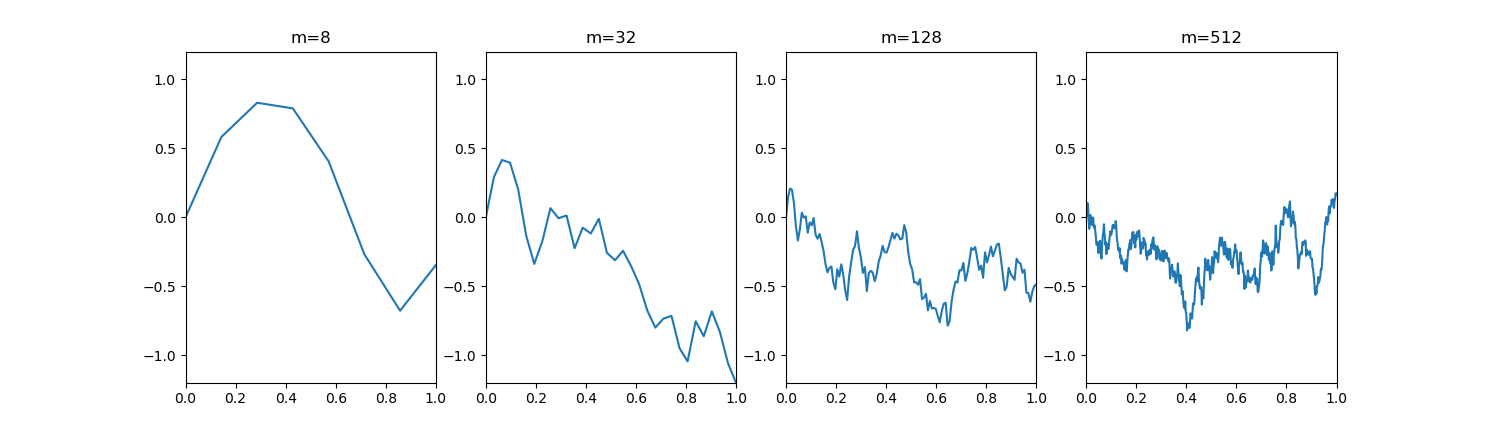
\includegraphics[scale=0.25]{Ben/DonskerBilder.png}
	\end{itemize}
	
\end{frame}


\begin{frame}
	\frametitle{SDE als ODE mit Random Walk}
	\begin{itemize}
		\item eindimensionale SDE:
		\begin{align*}
		& dX_t = \bm{\mu}(t,X_t) \, dt + \sum\limits_{j=1}^n \bm{\sigma}^{j}(t,X_t) \, dW^j
		\end{align*}
		\item Ito-Diffusion (nicht Zeit-abhängig):
		\begin{align*}
		& dX_t = \bm{\mu}(X_t) \, dt + \sum\limits_{j=1}^n \bm{\sigma}^{j}(X_t) \, dW^j
		\end{align*}
		\item Euler-Maruyama-Verfahren um Lösung $X$ zu approximieren:
		\begin{align*}
		& X_{m,t_k} := X_{m,t_{k-1}} + \Delta t^m \bm{\mu}(X_{m,t_{k-1}}) + \sqrt{\Delta t^m} \sum\limits_{j=1}^n \bm{\sigma^j}(X_{m,t_{k-1}})
		\end{align*}
		Für $0=t_0<...<t_m=\tau$ mit $t_k = k \frac{\tau}{m}$ und $\Delta t^m = \frac{\tau}{m}$.
	\end{itemize}
	
\end{frame}


\begin{frame}
	\frametitle{Lernen von $\bm{\mu}(0)$ und $\bm{\sigma}(0)$}
	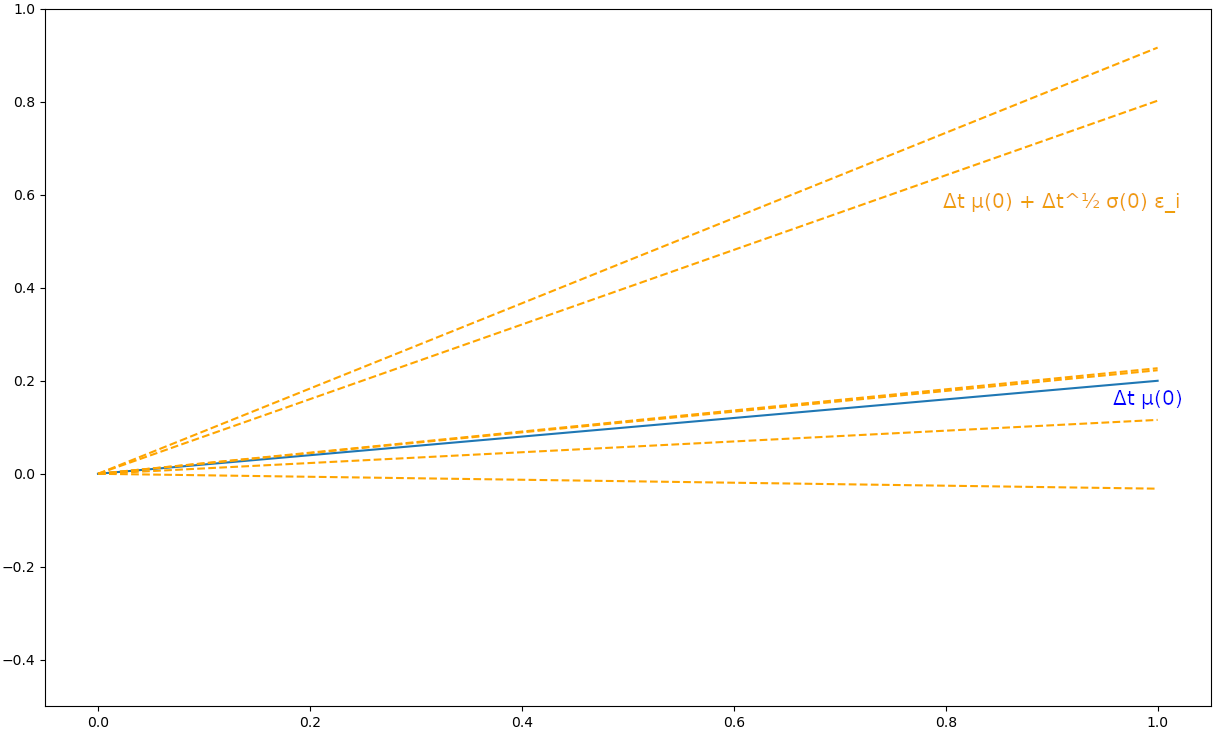
\includegraphics[scale=0.3]{Bilder/SDE_Erklaerung.png}
	
\end{frame}


\begin{frame}
	\frametitle{SDE-VAE Modell für $M=1$}
	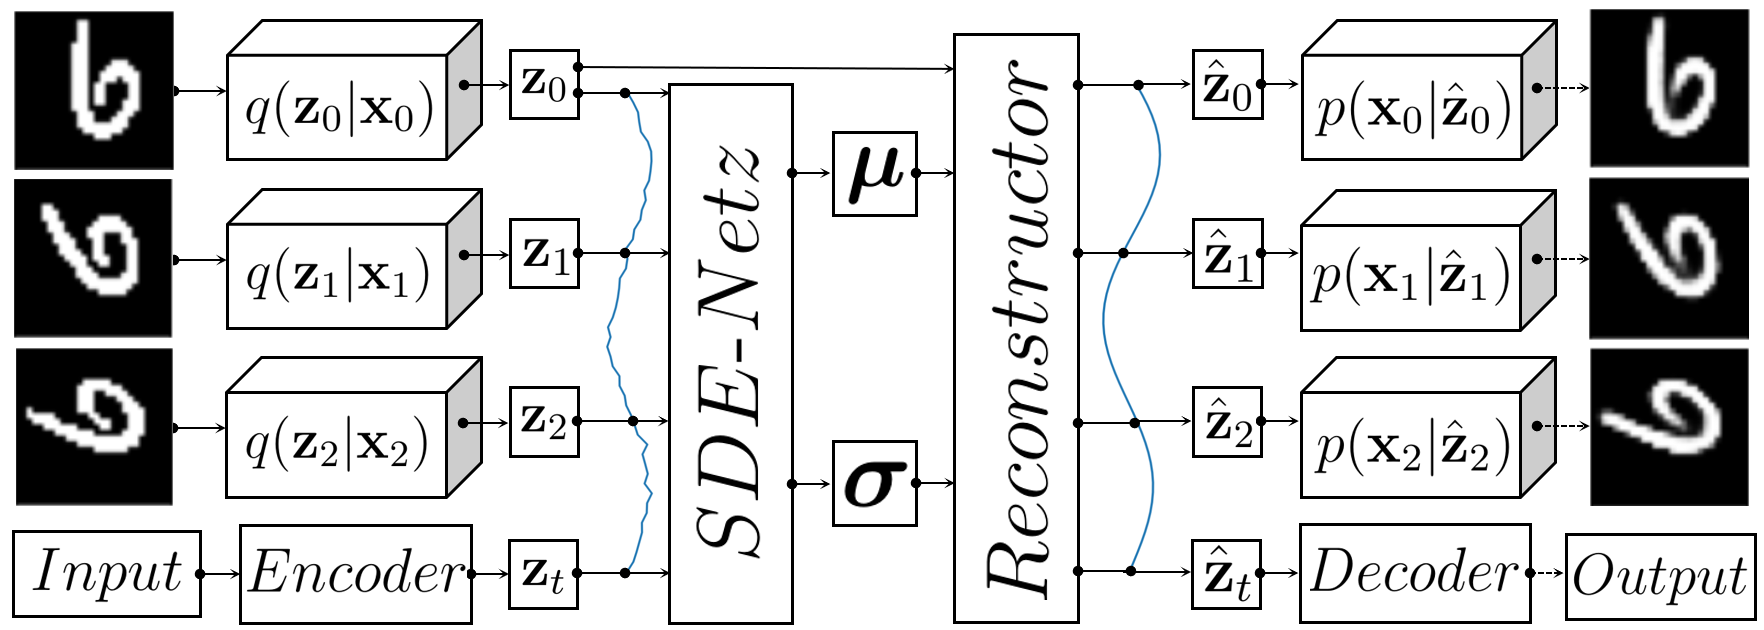
\includegraphics[scale=0.3]{Bilder/SDEVAEGrafik.png}
\end{frame}


\begin{frame}
	\frametitle{Ergebnisse}
	Einfaches Beispiel (mit $X_0 = (0,1)$)
	\begin{align*}
	& dX^1_t = X^2_t \, dt + 0,2 \, dW^1_t\\
	& dX^2_t = -X^1_t \, dt + 0,1 \, dW^1_t
	\end{align*}
	\begin{itemize}
		\item Lösungen für $X^1$:\\
		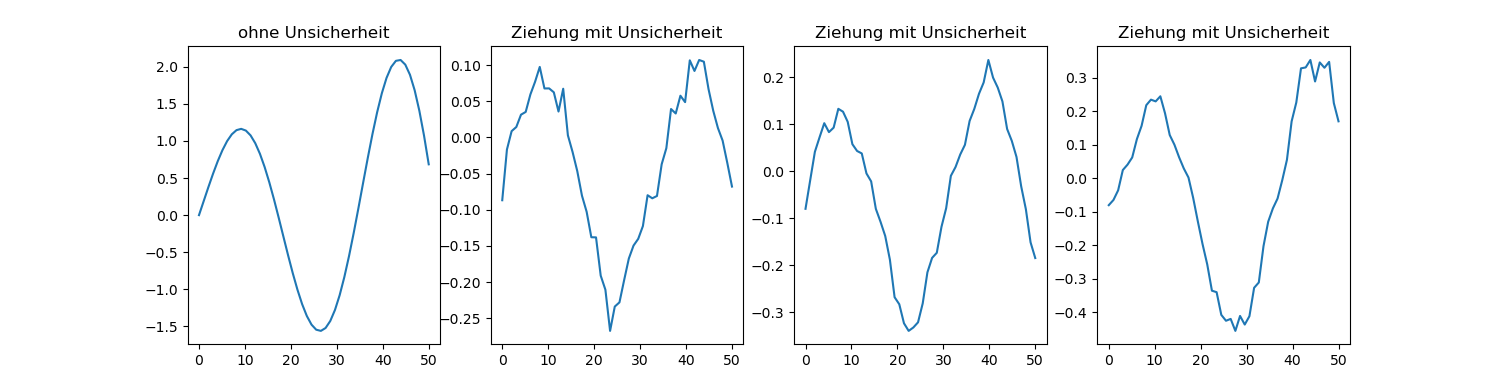
\includegraphics[scale=0.28]{Bilder/SDE_Loesungen.png}
		
		\item Rekonstruktionen nach gelernten $\bm{\mu}$ und $\bm{\sigma}$:\\
		%\includegraphics[scale=0.28]{Bilder/SDE_Rec.png}
		TODO
	\end{itemize}
	
\end{frame}


\begin{frame}
	\frametitle{Ergebnisse}
	
\includegraphics[scale=0.4]{Bilder/SDE_rotMNIST_rec}
\end{frame}

\begin{frame}
	\frametitle{Ergebnisse}
	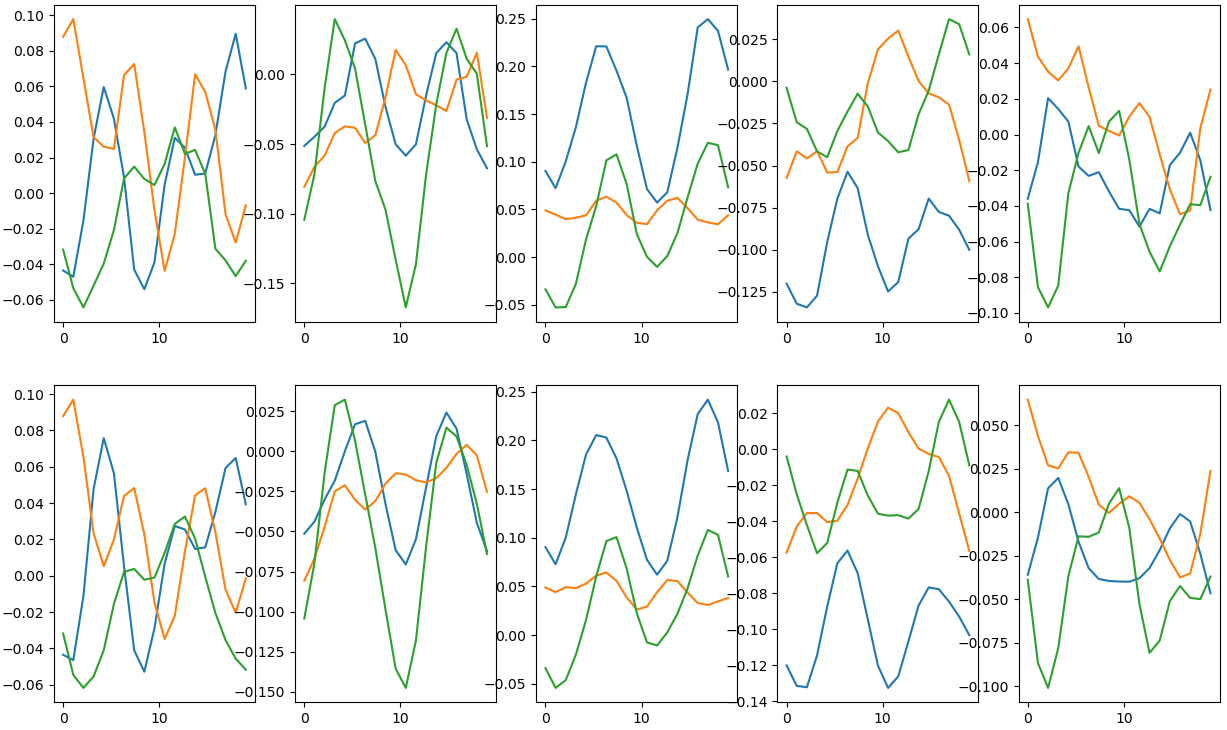
\includegraphics[scale=0.3]{Bilder/SDE_rotMNIST_latent_three_rec}
\end{frame}

















	\begin{frame}
		\frametitle{Quellen und Verweise}
		\begin{thebibliography}{9}
			\bibitem{vae}
			Diederik P. Kingma, Max Welling,
			\textit{Auto-Encoding Variational Bayes},
			2013,\\
			arXiv:1312.6114v10
			
			\bibitem{intvae}
			Diederik P. Kingma, Max Welling,
			\textit{An Introduction to Variational Autoencoders},
			2019,
			arXiv:1906.02691v3
			
			\bibitem{ode2vae}
			Çağatay Yıldız, Markus Heinonen, Harri Lähdesmäki,
			\textit{ODE$^{\ 2}$-VAE: Deep generative second order ODEs with Bayesian neural networks},
			2019,
			arXiv:1905.10994v2
		\end{thebibliography}
		\hfill\break
		\centering
		Vielen Dank für Ihre Aufmerksamkeit!
	\end{frame}
	
\end{document}
